\chapter{\label{method}PID controller using python}

\section{package: TCLab}

\begin{wrapfigure}{r}{0.5\textwidth} 
    \centering
    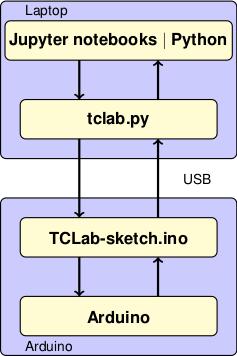
\includegraphics[width=0.5\textwidth]{TCLabOverview.png}
\end{wrapfigure}
The Arduino Temperature Control Lab is a modular, portable, and inexpensive solution for hands-on process control learning. Heat output is adjusted by modulating current flow to each of two transistors. Thermistors measure the temperatures. Energy from the transistor output is transferred by conduction and convection to the temperature sensor. The dynamics of heat transfer provide rich opportunities to implement single and multivariable control systems. The lab is integrated into a small PCB shield which can be mounted to any Arduino or Arduino compatible microcontroller.

\subsection{TCLab Overview}




The tclab package provides a set of Python tools for interfacing with the BYU Temperature Control Laboratory. The Temperature Control Laboratory consists of two heaters and two temperature sensors mounted on an Arduino microcontroller board. Together, the tclab package and the Temperature Control Laboratory provide a low-cost experimental platform for implementing algorithms commonly used for process control.

\subsection{TCLab Architecture}

\begin{wrapfigure}{r}{0.5\textwidth} 
    \centering
    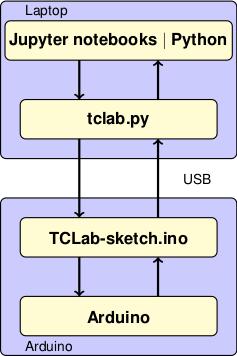
\includegraphics[width=0.5\textwidth]{TCLabOverview2.png}
\end{wrapfigure}

The tclab package is intended to be used as a teaching tool. The package provides high-level access to sensors, heaters, a pseudo-realtime clock. The package includes the following Python classes and functions:

\begin{itemize}
    \item TCLab() : providing access to the Temperature Control Laboratory hardware.
    \item TCLabModel() : providing access to a simulation of the Temperature Control Laboratory hardware.
    \item clock : for synchronizing with a real time clock.
    \item     Historian : for data logging.
    \item     Plotter : for realtime plotting.


\end{itemize}

    Using these Python tools, students can create Jupyter notebooks and python codes covering a wide range of topics in process control.

    \textbf{tclab.py:} A Python package providing high-level access to sensors, heaters, a pseudo-realtime clock. The package includes TCLab() providing access to the device, clock for synchronizing with a real time clock, Historian for data logging, and Plotter for realtime plotting. 

    \textbf{TCLab-sketch.ino:} Firmware for the intrisically safe operation of the Arduino board and shield. The sketch is available at https://github.com/jckantor/TCLab-sketch.

    \textbf{Arduino:}  Hardware platform for the Temperature Control Laboratory. TCLab is compatiable with Arduino Uno, Arduino Leonardo, and compatible clones.


\section{code}

\begin{minted}[
    frame=lines,
    framesep=2mm,
    baselinestretch=1.2,
    bgcolor=LightGray,
    fontsize=\footnotesize,
    linenos
    ]{python}
    import numpy as np
        
    def incmatrix(genl1,genl2):
        m = len(genl1)
        n = len(genl2)
        M = None #to become the incidence matrix
        VT = np.zeros((n*m,1), int)  #dummy variable
        
        #compute the bitwise xor matrix
        M1 = bitxormatrix(genl1)
        M2 = np.triu(bitxormatrix(genl2),1) 
    
        for i in range(m-1):
            for j in range(i+1, m):
                [r,c] = np.where(M2 == M1[i,j])
                for k in range(len(r)):
                    VT[(i)*n + r[k]] = 1;
                    VT[(i)*n + c[k]] = 1;
                    VT[(j)*n + r[k]] = 1;
                    VT[(j)*n + c[k]] = 1;
                    
                    if M is None:
                        M = np.copy(VT)
                    else:
                        M = np.concatenate((M, VT), 1)
                    
                    VT = np.zeros((n*m,1), int)
        
        return M
    \end{minted}



\begin{minted}[
    frame=lines,
    framesep=2mm,
    baselinestretch=1.2,
    bgcolor=LightGray,
    fontsize=\footnotesize,
    linenos
    ]{python}
    def PID(Kp, Ki, Kd, MV_bar=0):
    # initialize stored data
    e_prev = 0
    t_prev = -100
    I = 0
    
    # initial control
    MV = MV_bar
    
    while True:
        # yield MV, wait for new t, PV, SP
        t, PV, SP = yield MV
        
        # PID calculations
        e = SP - PV
        
        P = Kp*e
        I = I + Ki*e*(t - t_prev)
        D = Kd*(e - e_prev)/(t - t_prev)
        
        MV = MV_bar + P + I + D
        
        # update stored data for next iteration
        e_prev = e
        t_prev = t

    \end{minted}

\begin{minted}[
    frame=lines,
    framesep=2mm,
    baselinestretch=1.2,
    bgcolor=LightGray,
    fontsize=\footnotesize,
    linenos
    ]{python}


    %matplotlib inline
    from tclab import clock, setup, Historian, Plotter
    
    TCLab = setup(connected=False, speedup=10)
    
    controller = PID(2, 0.1, 2)        # create pid control
    controller.send(None)              # initialize
    
    tfinal = 800
    
    with TCLab() as lab:
        h = Historian([
            ('SP', lambda: SP), 
            ('T1', lambda: lab.T1), 
            ('MV', lambda: MV), 
            ('Q1', lab.Q1)])
        p = Plotter(h, tfinal)
        T1 = lab.T1
        for t in clock(tfinal, 2):
            SP = T1 if t < 50 else 50           # get setpoint
            PV = lab.T1                         # get measurement
            MV = controller.send([t, PV, SP])   # compute manipulated variable
            lab.U1 = MV                         # apply 
            p.update(t)                         # update information display
    \end{minted}




\section{Observation}

\newcommand{\plot}[3]{
\subsubsection{Seting the values of $K_p = #1$ , $K_i = #2 $ $K_d = #3$ we get the plot.}
\begin{figure}[H]
    \includegraphics[width= \linewidth]{PID(#1,#2,#3).png}
    \caption{PID(#1,#2,#3)}{
        
 \textbf{SP} Target temperature.
 \textbf{T1} Current temperature.
 \textbf{MV} Calculated power by PID.
 \textbf{Q1} Power on the heater coil.
    }
\end{figure}
}

\plot{2}{0.1}{2}
\plot{0.2}{0.1}{2}
\plot{2}{2}{2}
\plot{2}{20}{2}
\plot{10}{0.1}{2}
\plot{20}{0.1}{2}


\setcounter{equation}{0}
\setcounter{table}{0}
\setcounter{figure}{0}
%\baselineskip 24pt


    



